\documentclass[10pt,a4paper]{article}
\usepackage[utf8]{inputenc}

\usepackage{amsmath}
\usepackage{amsfonts}
\usepackage{amssymb}
\usepackage{graphicx}
\usepackage{listings}
\usepackage[margin=1.0in]{geometry}
\usepackage{caption}
\usepackage{subcaption}
\usepackage{float}
\usepackage[utf8]{inputenc}
\usepackage{refstyle}


\lstset{numbers=left,
	title=\lstname,
	numberstyle=\tiny, 
	breaklines=true,
	tabsize=4,
	language=Python,
	morekeywords={with,super,as},,
	frame=single,
	basicstyle=\footnotesize\tt,
	commentstyle=\color{comment},
	keywordstyle=\color{keyword},
	stringstyle=\color{string},
	backgroundcolor=\color{background},
	showstringspaces=false,
	numbers=left,
	numbersep=5pt,
	literate=
		{æ}{{\ae}}1
		{å}{{\aa}}1
		{ø}{{\o}}1
		{Æ}{{\AE}}1
		{Å}{{\AA}}1
		{Ø}{{\O}}1
	}
\usepackage{setspace}
\doublespacing
\usepackage{bm}
\usepackage{hyperref}

\begin{document}'
\begin{center}
{\LARGE\bf
FYS4150\\
Project 4 - deadline November 15
}
\\
 
\includegraphics[scale=0.1]{uio.png}\\
Sander W. Losnedahl\\
University of Oslo, Autumn 2017
 
\end{center}
\newpage

\begin{center}
{\LARGE\bf Introduction}
\end{center}

\newpage

\begin{center}
{\LARGE\bf Method}
\end{center}

\noindent To be able to start programming, one first needs to find the expressions for the partition function $Z$ with its corresponding energy values $E$, the mean magnetic moment $M$, the specific heat $C_V$ and the susceptibility $X$ as functions of the temperature $T$. All of this using the periodic boundary condition.
\\
The partition function $Z$ is giving by: 


$$
Z = \sum^{M}_{i = 1} e^{-\beta * E_i}
$$ 

\noindent where $\beta$ is the inverse temperature given by $\beta = \frac{1}{kT}$ where k is the Boltzmann constant and T is the temperature, so every expression with $\beta$ beneath is dependent on the temperature $T$. $E_i$ is the energy for different spin settings given by:

$$
E = -J\sum^{N}_{<kl>} s_ks_l
$$

\noindent where J is the coupling constant and N is the total number of spins. $s_k$ and $s_l$ are the spins of two neighbouring objects in a lattice. Since we are working 2x2 lattice, the total number of combinations are given by $2^4 = 16$, considering we are working with the Ising model where the spins can only be $-1$ or $1$.
\\
\begin{figure}[H]
\centering
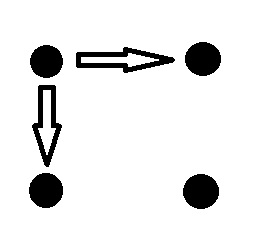
\includegraphics[width=0.5\textwidth]{22lattice}
\caption{A two by two lattice and how they interact using the Ising model}
\label{fig:22lattice}
\end{figure}
\noindent From \figref{22lattice} we see how the Ising model works on a 2x2 lattice and from this the energy is calculated. One can observe that energy is non-zero on lattices where all the objects have the same spin ($-8J$) and where the two diagonals have opposite spin from each other ($8J$). All other settings have zero energy. Lets calculate the energy where the diagonals have opposite spin to see how this works:

$$
E = -J((1*-1 + 1*-1) + (-1*1 + -1*1) + (1*-1 + 1*-1) + (-1*1 + -1*1))
$$
$$
E = -J(-8) = 8J
$$

\noindent Now we can simply put the energy values into our partition function:

$$
Z = e^{-\beta * -8J} + e^{-\beta * -8J} + e^{-\beta * 8J} + e^{-\beta * 8J} + 12*e^0
$$
$$
Z = 2e^{-8J\beta} + 2e^{8J\beta} + 12
$$

\noindent The magnetization is given by:

$$
M = \sum^{N}_{j = 1} s_j
$$

\noindent Unlike in the energy case, the magnetization does not depend the lattice having the same spin or that the diagonals have opposite spin. The only case where the magnetization is zero in a 2x2 lattice is when half of the objects in the lattice have negative and the other half having positive spin. Therefore we get the magnetization values:

$$
M_i = [4 + 2 + 2 + 2 + 2 + 0 + 0 + 0 + 0 + 0 + 0 + -2 + -2 + -2 + -2 + -4] = 0
$$

\noindent The sum of these are zero, which makes sense since these values represent all possible spin settings. To calculate the mean magnetic moment or mean magnetization we use the equation:

$$
|M| = \frac{1}{Z}\sum^{M}_{i}M_ie^{-\beta E_i}
$$
\\
\noindent The mean magnetization would also be zero since we still sum all of the possible spin settings with the previously mention energy values. The specific heat is given by:

$$
C_V = (N-1)k(\frac{\beta J}{cosh(\beta J})^2
$$
which already depend on $\beta$ and therefore temperature, so we don't need to rewrite the expression in any way.
\\
To calculate the susceptibility, one has to first calculate the the variance of the mean magnetization given by

$$
\sigma_M^2 = <M^2>-<M>^2 = \frac{1}{Z}\sum^{M}_{i = 1}M_i^2 e^{-\beta E_i} - (\frac{1}{Z}\sum^{M}_{i = 1}M_i e^{-\beta E_i})^2
$$

\noindent We immediately observe that the second term in the above equation is equal to 0 because the sum of all magnetization is 0. However, the first term is not equal to zero because the magnetization is squared. This gives us a variance of:

$$
\sigma^2 = \frac{32}{Z}(e^{8J\beta}+1)
$$

\noindent Now we can calculate the susceptibility given by:

$$
X = \frac{1}{k_bT}(<M^2> - <M>^2) = \frac{1}{k_bT}\sigma^2 = \frac{32}{Zk_bT}(e^{8J\beta}+1)
$$










\end{document}